\chapter{Quantum Fourier Transform}

\section{Introduction to the Discrete Quantum Fourier Transform}

The discrete fourier transform on a vector $x = \left( x_0, x_1 \cdots x_{n-1} \right)$ is given by the vector $y = \left(y_{0}, y_1 \cdots y_{n-1} \right)$ where we have
$$ y_j = \frac{\sum_{k=0}^{n-1} x_k \exp(\frac{2\pi ijk}{n})}{\sqrt{n}}$$

Analogously we can define the discrete fourier transform of our quantum hilbert space of $n$ qubits by the linear operator that takes our basis states $\ket{j} \in \{ \ket{0}, \ket{1} \cdots \}$ to the state given by
$$ \ket{j} \to \frac{1}{\sqrt{2^n}}\sum_{k=0}^{n-1} \exp(\frac{2\pi ijk}{n}) \ket{k}} $$

\begin{exercise}
Prove that the above transformation is unitary
\end{exercise}

\begin{exercise}
Prove that the above quantum unitary operation achieves the discrete fourier transform as defined for a sequence/vector as given above.
\end{exercise}

We state the following compact form for the fourier transform for our quantum hilbert space which makes it easier to construct a circuit to achieve the quantum fourier transform. This follows by some basic algebra which we leave as an exercise.

$$ \ket{j_1, j_2 \cdots j_n} \to \frac{\left(\ket{0} + e^{2\pi i0.j_n}\ket{1} \right)\left(\ket{0} + e^{2\pi i0.j_{n-1}j_n}\ket{1} \right) \cdots \left(\ket{0} + e^{2\pi i0.j_{1}j_{2}\cdots j_{n}}\ket{1} \right)}{\sqrt{2^n}}$$

The circuit below computes the quantum fourier transform

\begin{figure}[htp]
    \centering
    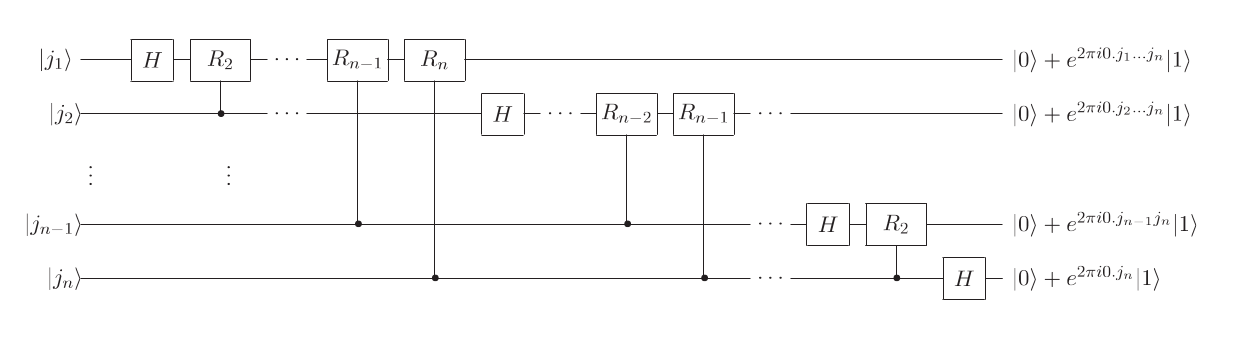
\includegraphics[width=\textwidth]{qft}
\end{figure}

where $R_k$ is defined to be the gate acting on a single qubit given by the matrix
$$R_k = \begin{bmatrix}
1 & 0 \\
0 & e^{2\pi i/2^k} 
\end{bmatrix}$$

To see why observe that the hadamard gate on a qubit $\ket{j_1}$ changes it to
$$\ket{j_1} \to \frac{\left( \ket{0} + e^{2\pi 0.j_1}\ket{1} \right)}{\sqrt{2}}$$

Successive applications of the controlled $R$ gates then finally take $\ket{j_1}$ to 
$$\ket{j_1} \to \frac{\left( \ket{0} + e^{2\pi 0.j_{1}j_{2}\cdots j_{n}}\ket{1} \right)}{\sqrt{2}}$$

We repeat the same process with the other input bits and then take their tensor product to get the form of quantum fourier transform that we obtained above. Notice that we will have to use swap gates (cross over gates that swap qubits) in order to obtain the order given in the compact form above.

Notice that we needed gates in the order of $n^2$ to do the above operation. Thus the Quantum Fourier Transform requires $O(n^2)$ operations to finish where the operation of one single qubit gate is taken as a constant. This is a massive improvement over the classical algorithms which require exponential gates to finish.

Now we will look at some applications of Quantum Fourier Transform, beginning with Phase Estimation.

\section{Phase Estimation}
Using Quantum Fourier Transform we can easily estimate the phase of the eigenvalue of a unitary operator. Recall that unitary operators have eigenvalues whose absolute value is one. Thus for any unitary operator $U$ has it's eigenvalues in the form $e^{i\varphi}$. For now we assume that we have a way of preparing an eigenstate of $U$ $\ket{u}$ with eigenvalue $e^{2\pi i\varphi}$. Thus,
$$ U\ket{u} = e^{2\pi i\varphi}\ket{u}$$
For now suppose that $\varphi$ in binary can be written in the form $0.\varphi_{1}\varphi_{2}\cdots\varphi_{n}$ exactly. That is,
$$\varphi = \sum_{i=1}^{n} \frac{\varphi_{i}}{2^{i}} $$ The following circuit can be used to find $\varphi$

\begin{figure}[htp]
    \centering
    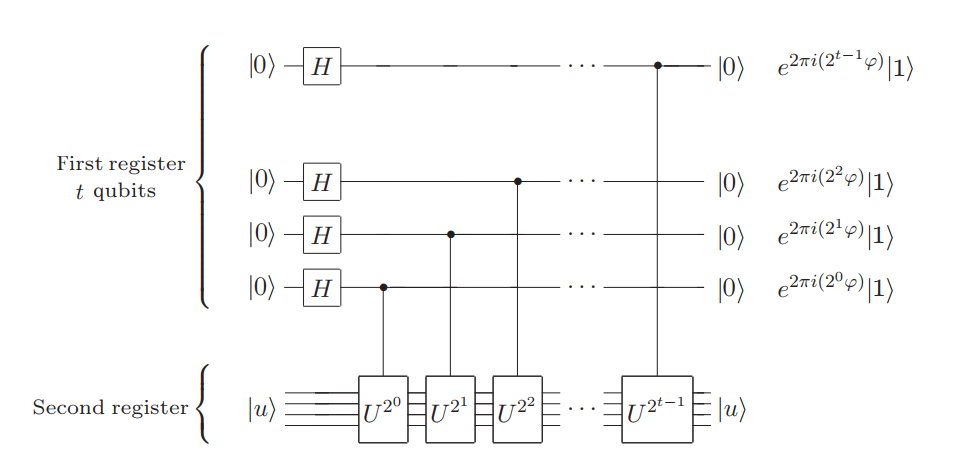
\includegraphics[width=\textwidth]{phase}
\end{figure}

Here we are using the controlled $U^{2^j}$ operation on the second register with the control bits being the t qubits in the control register. Suppose the control qubit is given by $\ket{\psi} = \alpha\ket{0} + \beta\ket{1}$ Observe that when the controlled $U^{2^j}$ operation acts on the second register which is fed in an eigenstate $\ket{u}$ of $U$ it causes the control qubit to change to $\alpha\ket{0} + \beta e^{2\pi i2^{j}\varphi}\ket{1}$. Using this prove the following:
\begin{exercise}
Prove that the final state of the first register in the above circuit will be $$\frac{1}{2^{t/2}}\left( \ket{0} + e^{2\pi i2^{t-1}\varphi}\ket{1} \right)\left( \ket{0} + e^{2\pi i2^{t-2}\varphi}\ket{1} \right) \cdots \left( \ket{0} + e^{2\pi i\varphi}\ket{1} \right) = \sum_{k=1}^{2^t - 1} \frac{1}{2^{t/2}}e^{2\pi i\varphi k}\ket{k}$$
\end{exercise}

Observe that the left hand side of the above final state can be written in the form $$\frac{1}{2^{t/2}}\left( \ket{0} + e^{2\pi i0.\varphi_{t}}\ket{1} \right)\left( \ket{0} + e^{2\pi i0.\varphi_{t-1}\varphi_{t}}\ket{1} \right) \cdots \left( \ket{0} + e^{2\pi 0.\varphi_{1}\varphi_{2}\cdots\varphi_{t}}\ket{1} \right)$$

But this is precisely the result we obtain by taking the quantum fourier transform of the state $\ket{\varphi_{1}\varphi_{2} \cdots \varphi_{t}}$. Thus is we take the inverse fourier transform of the above circuit we will end up with $\ket{\varphi_{1}\varphi_{2} \cdots \varphi_{t}}$ thus giving us the phase.

However in general the phase may not be exactly expressible in $t$ qubits. But it seems intuitive that if use more qubits in the first register then we should be able to get a pretty good estimate of the phase. Indeed this is the case and the following theorem which we state without proof (readers are encouraged to refer to the textbook or wikipedia for details) gives us a quantitative bound on the number of qubits we should use in the first register.

\begin{theorem}
Suppose we desire to obtain the phase $\varphi$ up to an accuracy of $2^{-n}$ with probability of success atleast $1 - \epsilon$ then we should take $t$ qubits in the first register where $t$ is given by
$$ t = n + \left \lceil{\log(2 + \frac{1}{2\epsilon})}\right \rceil $$
\end{theorem}

Notice that after using the above $t$ qubits we should only consider the values in the first $n$ registers. Now that we know how to estimate the phase we can use it to to find the order of a number modulo $N$ and use this to factorise a number. Let's discuss this in detail.

\section{Order Estimation}
The order of a number $x$ modulo $N$ is defined as the least $r$ such that $$ x^r \equiv 1  \mod N$$ Clearly this makes sense only when $\gcd(x, N) = 1$
\begin{exercise}
Prove that $r \leq \phi(N)$
\end{exercise}

On a classical computer it is believed that the order estimation problem is not in $\textbf{P}$ that is there exists no polynomial time algorithm in $L \equiv \left \lceil{ \log(N)} \right \rceil$ which can be used to find the order. We will now use phase estimation to describe such a quantum polynomial algorithm.
For a fixed $x$ let us define a unitary operator $U$ satisfying 
$$U\ket{y} = \ket{xy \Mod{N}}$$ where $y \in \{0, 1\}^L$ with the convention that for $y \geq N$, $\ket{xy \Mod{N}} = y$

\begin{exercise}
Prove that the above operator U is indeed unitary
\end{exercise}
\begin{solution}
Observe that any operator acting on our quantum hilbert space that satisfies the length normalisation condition has to be unitary (why?).
Now observe that the above transformation maps basis vectors to basis vectors and hence must satisfy the length normalisation condition (that is if $\braket{\psi}{\psi} = 1$ then $\braket{U\psi}{U\psi} = 1$) and thus $U$ is unitary.
\end{solution}

Consider the states defined by
$$ \ket{u_s} = \frac{1}{\sqrt{r}} \sum_{k=0}^{r-1} \exp[\frac{-2\pi isk}{r}] \ket{x^k\Mod{N}}$$
\begin{exercise}
Prove that the above states are eigenstates of $U$.
\end{exercise}

We can see that the eigenvalues of the above eigenstate $\ket{u_s}$ will be $\exp(\frac{2\pi is}{r})$. Therefore phase estimation will allow us to find an approximation to $s/r$ upto the number of qubits we desire. Then we will use the continued fractions algorithm to obtain $r$ (more on that later).

This however is not as easy. Firstly we have no way to prepare an eigenstate of $U$. Fortunately we can use the following fact
\begin{exercise}
Prove that $$\frac{1}{\sqrt{r}} \sum_{s=0}^{r-1} \ket{u_s} = \ket{1}$$
\end{exercise}

This is useful because now instead of passing in $\ket{u_s}$ in the second register we can pass in $\ket{1}$. Then by linearity the output after inverse fourier transform will be 
$$ \sum_{s=0}^{r-1} \frac{1}{\sqrt{r}}\ket{\phi_s}\ket{u_s} $$ where $\phi_s$ is an approximation to $s/r$. Now when we start measuring the first register we will finally obtain the binary representation of $s/r$ where $s$ will be a whole number less than $r$ and the probability of $s$ equaling any such number will be the same for all (as the coefficients across the eigenstates are the same). Infact if we use Theorem 10.1 the probability will be modified to become $\left ( 1 -\epsilon \right)/r$.

We will be wanting an accuracy of $2L + 1$ qubits in our estimate as we will see later. Clearly the number of gates needed will be $O(L^2)$ for the inverse fourier transform. For the phase estimation observe that we would also need an efficient way to do controlled $U^{2^j}$ operations. This can be shown to be done with $O(L^3)$ gates using modular exponentation. Thus so far we need $O(L^3)$ gates to perform the phase estimation.
\begin{figure}[htp]
    \centering
    \caption{Circuit for Order Estimation}
    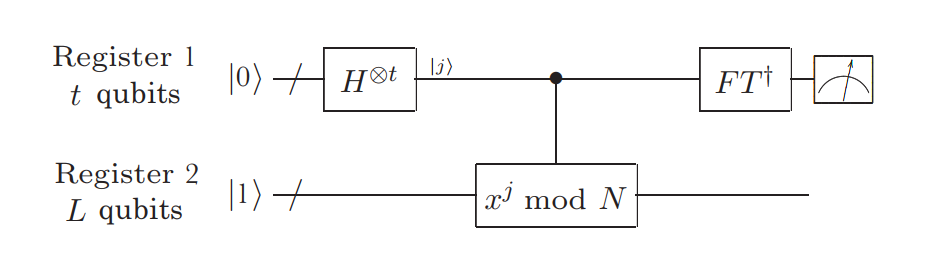
\includegraphics[width=\textwidth]{order}
\end{figure}

Now to extract $r$ from $s/r$ we will use the continued fractions algorithm. The following theorem becomes incredibly useful

\begin{theorem}
Let $s/r$ be a rational number such that for another rational number $\phi$ it satisfies 
$$ |\frac{s}{r} - \phi| \leq \frac{1}{2r^2}$$
Then $s/r$ is a convergent of the continued fractions expansion of $\phi$
\end{theorem}

\begin{exercise}
Prove that the above condition is held for our $\phi$ being the approximation to $s/r$ upto $2L + 1$ digits.
\end{exercise}

Thus taking our estimate $\phi$ and finding it's continued fraction expansion will allow us to evaluate all the convergents of this continued fraction.

As a recap continued fractions allow us to represent any number $x$ in the form $\left[ a_0, a_1, a_2 \cdots \right]$ where 
$$ x = a_0 + \frac{1}{a_1 + \frac{1}{a_2 + \frac{1}{\cdots}}} $$
In the case of rationals this set is finite. The convergent simply corresponds to select a prefix of this set, that is if the representation of the rational was $\left[ a_0, a_1, a_2 \cdots a_M \right]$  then the $mth$ convergent will simply be $\left[ a_0, a_1, a_2 \cdots a_m \right]$ where $m \leq M$.

This process also takes $O(L^3)$ gates and then we can simply evaluate all the candidates for $s/r$. Now as we have an exact value for $r$ we can simply check if this is the order or not. Note that if some value of $r$ does satisfy $x^r \equiv 1 \pmod N$ then it must be the order and not a multiple of it (why?). There could be one issue and and that is if $s$ and $r$ have common factors then the continued fractions algorithm will give us $s'$, $r'$ such that $s'/r'$ = $s/r$. But this isn't an issue because the probability of $s$ and $r$ being coprime is high and so we can simply run the process multiple times until we get the value of $r$ that we seek.

Thus we have found the order of $x$ modulo $N$ using only $O(L^3)$ gates. This we shall see will become very useful in factoring numbers as this is a routine used in Shor's algorithm.

\section{Shor's Algorithm}
\begin{figure}[htp]
    \caption{Circuit for Shor's algorithm}
    \centering
    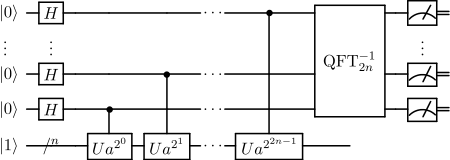
\includegraphics[width=\textwidth]{shor}
\end{figure}
Shor's algorithm for factoring uses the order finding algorithm that we described above to factorise a number. All the other step's in Shor's algorithm can be done using a classical computer efficiently and thus it is the quantum order finding subroutine that is the main component of Shor's algorithm.

We can reduce the factoring problem to the order finding problem. We will show this equivalence using a few theorems. First consider the following interesting theorem

\begin{theorem}
Suppose $N$ is an $L$ bit composite number, and $x$ is a non-trivial solution to the equation $x^2 \equiv  1 \pmod N$ in the range $1 \leq x \leq N$, that is, neither $x \equiv 1  \pmod N$ nor $x \equiv N - 1 \pmod N$. Then at least one of $\gcd(x − 1, N)$ and $\gcd(x + 1, N)$ is a non-trivial factor of $n$ that can be computed using $O(L^3)$ operations.
\end{theorem}
\begin{proof}
Left as exercise (hint: consider the negation and proceed by contradiction)
\end{proof}

Now suppose we have that $y$ is coprime to $N$ where $ 1 \leq y \leq N$ (else their greatest common divisor will be a divisor of $N$ thus giving us a factor and solving the factoring problem). Suppose the order of $y$ modulo $N$ is even and also satisfies $y^{r/2} \not\equiv -1 \pmod N$. Then we can set $x = y^{r/2}$ in the theorem above and so we can simply use this value to find a non trivial factor of $N$. This is the basic idea of Shor's algorithm. However we need to ensure the above two conditions. We can get a bound on the probability of this occurring and thus by repeating the process a couple of times we can with high probability get a factor. Notice that this is true assuming that the number is composite.

The following theorem gives a bound on the above conditions holding whose proof we omit as it involves generators and group theory.

\begin{theorem}
Suppose $N = p_1^{\alpha_{1}}p_2^{\alpha_{2}} \cdots p_m^{\alpha_m}$ is the prime factorization of an odd composite
positive integer. Let $x$ be an integer chosen uniformly at random, subject to the
requirements that $1 \leq x\leq N - 1$ and $x$ is co-prime to $N$. Let $r$ be the order of
$x$ modulo $N$. Then
$p(r$ is even and $x^{r/2} \equiv − 1 \pmod N ) \geq 1 - \frac{1}{2^m}$
\end{theorem}

Thus the probability of the above condition being satisfied increases as the number of distinct primes dividing our numbers increases. Thus by repeated applications we can ensure that our algorithm suceeds.\\

The summary of the algorithms is as follows:

Input: A composite number $N$
\\
Output: A non trivial factor of $N$
\\
Complexity: $O(\log^3 N)$, succeeds with probability $O(1)$\\
Steps:
\\
1. If $N$ is even return 2\\
2. Else take $x$ satisfying $1 \leq x \leq N-1$. If $\gcd(x, N)$ is not $1$ then return $\gcd(x, N)$\\
3. Else run the order finding algorithm to find the order $r$ of $x$ modulo $N$\\
4. Check if $r$ is even and $x^{r/2} \neq -1 \pmod N$. If this is satisfied compute $\gcd(x^{r/2} - 1, N)$ and $\gcd(x^{r/2} + 1, N)$ and return whichever of them is not equal to 1. If this is not satisfied the algorithm does not succeed.
\\\\
To ensure high probability of success we will run the algorithm multiple times.
This sums up Shor's algorithm and the usage of Quantum Fourier Transform. Quantum Fourier Transform can be used for various other applications like period estimation, discrete logarithm and a class of problems known as the hidden subgroup problem. The reader is encouraged to go through the textbook to study these topics in depth. Now we shall see how Quantum Search can be achieved using Grover's algorithm.
\clearpage